% v2-acmlarge-sample.tex, dated March 6 2012
% This is a sample file for ACM large trim journals
%
% Compilation using 'acmlarge.cls' - version 1.3, Aptara Inc.
% (c) 2011 Association for Computing Machinery (ACM)
%
% Questions/Suggestions/Feedback should be addressed to => "acmtexsupport@aptaracorp.com".
% Users can also go through the FAQs available on the journal's submission webpage.
%
% Steps to compile: latex, bibtex, latex latex
%
\documentclass[prodmode,acmtap]{acmlarge}

% Metadata Information
\acmVolume{2}
\acmNumber{3}
\acmArticle{1}
\articleSeq{1}
\acmYear{2013}
\acmMonth{11}

% Package to generate and customize Algorithm as per ACM style
\usepackage[ruled]{algorithm2e}
\SetAlFnt{\algofont}
\SetAlCapFnt{\algofont}
\SetAlCapNameFnt{\algofont}
\SetAlCapHSkip{0pt}
\IncMargin{-\parindent}
\renewcommand{\algorithmcfname}{ALGORITHM}

% Page heads
\markboth{J. Datko}{The Architecture of Tor}

% Title portion
\title{The Architecture of Tor}
\author{JOSHUA DATKO \affil{Drexel University}
}
% NOTE! Affiliations placed here should be for the institution where the
%       BULK of the research was done. If the author has gone to a new
%       institution, before publication, the (above) affiliation should NOT be changed.
%       The authors 'current' address may be given in the "Author's addresses:" block (below).
%       So for example, Mr. Fogarty, the bulk of the research was done at UIUC, and he is
%       currently affiliated with NASA.

% \category{H.5.2}{Information Interfaces and Presentation}{User
% Interfaces}[Evaluation/\break methodology]
% \category{H.1.2}{Models and Principles}{User/Machine Systems}[Human Information Processing]
% \category{I.5.1}{Pattern\break Recognition}{Models}[Neural Nets]

% \terms{Human Factors}
% \keywords{Contour perception, flow visualization, perceptual theory, visual cortex, visualization}

% \acmformat{Daniel Pineo, Colin Ware, and Sean Fogarty. 2010. Neural Modeling of Flow Rendering Effectiveness.}
% At a minimum you need to supply the author names, year and a title.
% IMPORTANT:
% Full first names whenever they are known, surname last, followed by a period.
% In the case of two authors, 'and' is placed between them.
% In the case of three or more authors, the serial comma is used, that is, all author names
% except the last one but including the penultimate author's name are followed by a comma,
% and then 'and' is placed before the final author's name.
% If only first and middle initials are known, then each initial
% is followed by a period and they are separated by a space.
% The remaining information (journal title, volume, article number, date, etc.) is 'auto-generated'.

\begin{document}



\begin{bottomstuff}
Author's email: jbd65@drexel.edu
\end{bottomstuff}


\maketitle

% Head 1
\section{Introduction}
Tor is an anonymizing, overlay network that has grown and evolved
substantially since its release in 2004.  However, it is much more
than a network.  It is a suite of protocols, free software, a
non-profit organization, and a software ecosystem.  While not
explicitly stated, Tor is a \emph{platform} that provides network
layer anonymization to a wide range of services.  Additionaly, there
are over thirty independent projects in the Tor ecosystem that range
from metrics gathering to web and email client plugins.  This paper
provides an architecture review of the Tor platform.  Section
\ref{overview} summarizes the Tor design.  Section \ref{detailed}
provides a detailed, layered view of Tor and finally, Section
\ref{quality} analyzes several architectural qualities of Tor.

\section{Functional Overview}\label{overview}
%BREIF overview of the platform/software that you are investigating
%What does it do?  How big is it?  What is the tech-stack (is it Java, Ruby, Java EE, etc)
%Produce a high-level view showing the overall architecture of the system
Tor is an overlay network that runs atop TCP.  The main deployment and
usage of Tor is shown in Figure \ref{fig:tor_deployment}.  The Tor
network is composed of Tor clients and Onion Routers (ORs).  ORs are
furthered classified as relays, exit relays, or bridges (not shown).
The most common use case for Tor is a user, Alice, who wants to visit
a website without revealing her Internet Protocol (IP) address to the
website.

\begin{figure}[h]
\centering
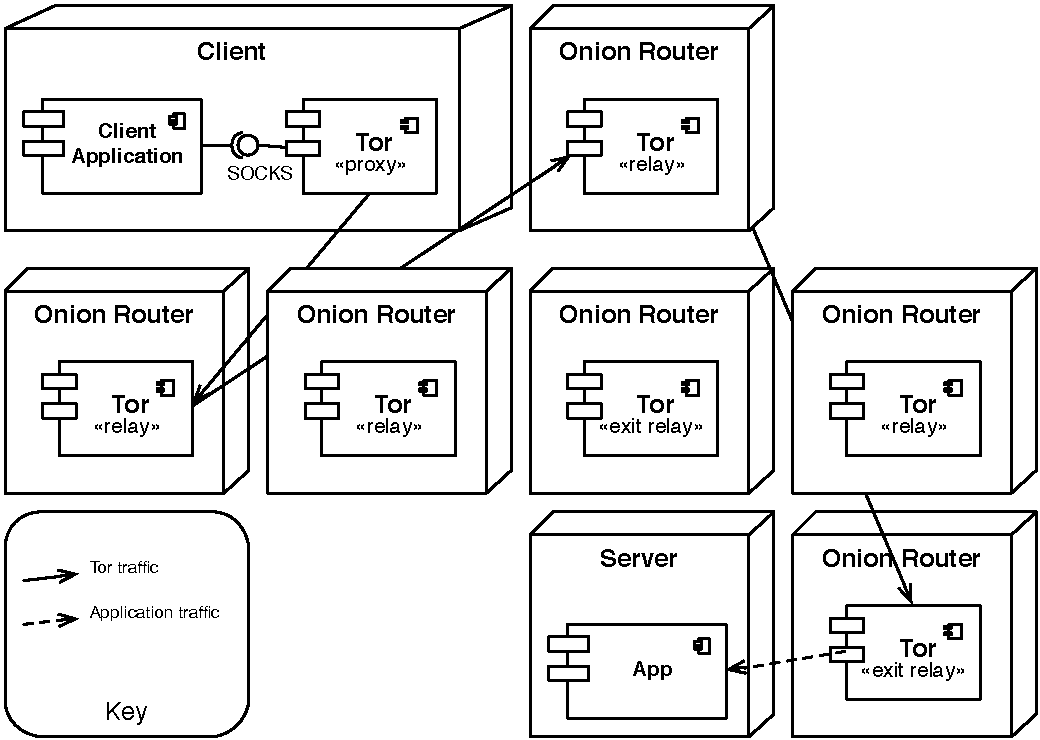
\includegraphics[width=0.5\textwidth]{tor_deployment.pdf}
\caption{Tor Deployment Diagram}
\label{fig:tor_deployment}
\end{figure}

Alice starts a local Tor instance on her computer, which offers a
Socket Secure (SOCKS) Proxy on her machine.  She then starts a browser
configured to use the local SOCKS Proxy.  Tor distributes a forked
version of Mozilla Firefox called the Tor Browser Bundle (TBB), that
is not only specifically configured to interact with the proxy, but
contains re-written portions of Firefox to protect anonymonity leaks.
For example, prior to connecting to a website, the client must perform
a Domain Name Server (DNS) lookup.  However, the DNS lookup exposes
the destination address and is counter productive to protecting
Alice's identity.

Alice's local Tor client chooses three nodes in the Tor network: a
guard node, a middle, and an exit node.  She encrypts the messages in
a layered approach.  The entire payload is encrypted to the guard
node.  The guard can decrypt the message, but that message simply
contains instructions to send the message to the middle node, which he
does.  The middle node decrypts the message, but that message tells
him to forward the remaining message to the exit.  When the exit
decrypts the message, it contains the actual data that Alice wants to
transmit to the destination and the exit nodes makes that connection
on behalf of Alice (via the middle node).  The exit does not know
Alice's IP address nor the address of the guard node, but he does know
the destination.  The middle node knows the IP addresses of the guard
and exit, but not of the destination nor Alice.  The guard knows
Alice's IP address and the middle node, but not the exit nor the
destination.  Hence the ``onion'' in Tor; each layer is peeled back by
each OR.

\subsection{Deployment Size}

As shown in Figure \ref{fig:network_size}, Tor is composed of roughly
4600 relays.  Tor is largely a volunteer network.  Relay operators
donate bandwidth and processing to support the Tor mission.  While
there are some paid servers (usually under a non-profit), the major of
Tor are altruistic volunteers.  Tor seems more impressive given the
number of users.  While Figure \ref{fig:user_size} shows roughly 4
million clients, about three million of these are suspected to be a
dormant botnet that has recently joined the network.

\begin{figure}[h]
\centering
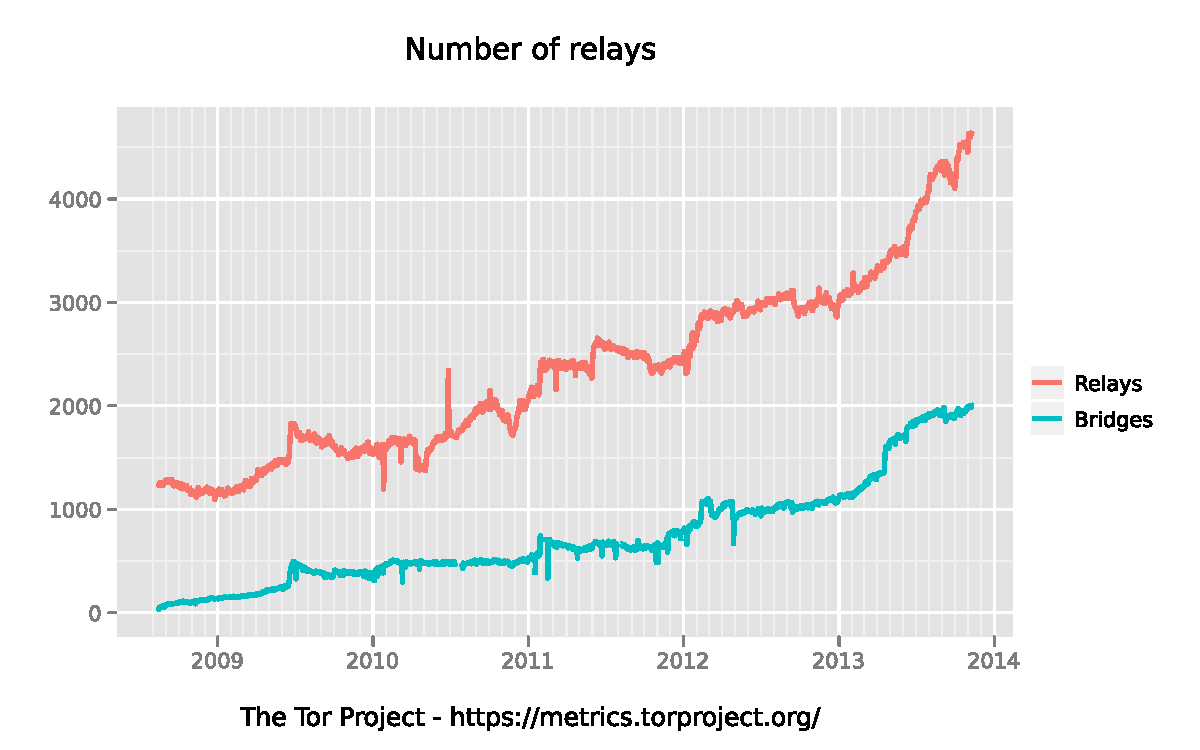
\includegraphics[width=0.5\textwidth]{networksize-2008-08-14-2013-11-12.pdf}
\caption{Tor Network Size}
\label{fig:network_size}
\end{figure}

\begin{figure}[h]
\centering
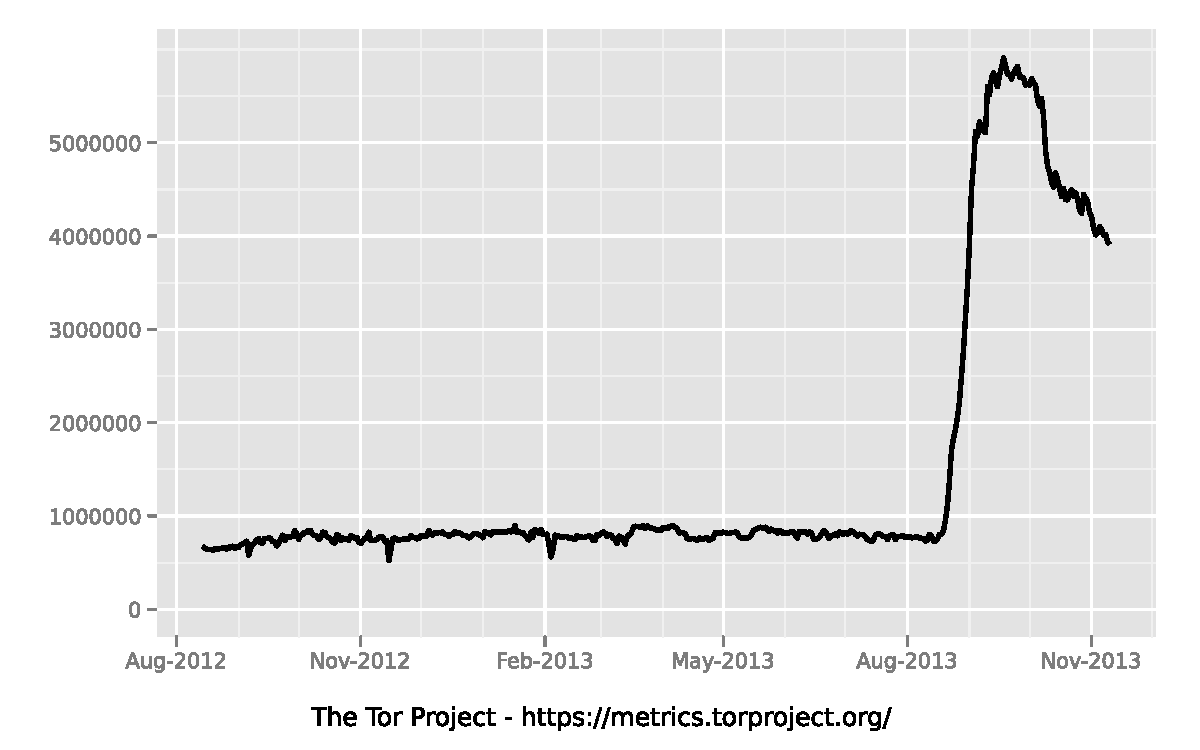
\includegraphics[width=0.5\textwidth]{userstats-relay-country-2012-08-14-off-2013-11-12-all.pdf}
\caption{Tor User Size}
\label{fig:user_size}
\end{figure}


\subsection{Tech Stack}

The core Tor software is written in C as it performs various low-level
networking and cryptographic functions mainly using OpenSSL.  However,
its external interface are well defined networking protocols,
therefore software that uses Tor services are language independent.
For example, there is a port of the Tor browswer that runs on Android OS.

\section{Detailed View}\label{detailed}
% How would you show and explain the architecture to somebody else in 20 minutes
% What other views?
% Why are they important?
% What are they showing that is important to improve understanding?
A key view to further understanding Tor is a layered view.  Figure \ref{fig:tor_layer}
shows the mapping of the protocols used in Tor to the OSI seven layer
network model.  Tor mainly exists at the session layer.  It provides a
SOCKS proxy as the initial interface.  The actual Tor network is a
fixed-cell circuit network, analogous to Asynchronous Transfer Mode
(ATM).  The Tor protocol establishes connections over Transport Layer
Security (TLS), and Tor traffic is pushed over these connections.

\begin{figure}[h]
\centering
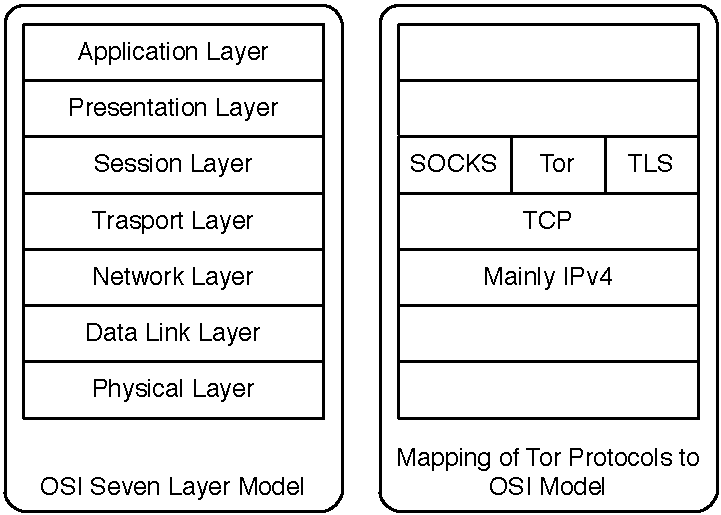
\includegraphics[width=0.5\textwidth]{tor_layer.pdf}
\caption{Tor Layered View}
\label{fig:tor_layer}
\end{figure}

The layered view is important because it shows the Tor does and does
not protect.  There are many misconceptions about the protection
provided by Tor.  Tor does not ``encrypt the Internet.''  In Figure
\ref{fig:tor_layer}, it is clear to see that Tor operates at the
network layer and can not provide confidentiality services to
Application data, once it has left the network layer.

\subsection{Patterns}

The architecture overview, Figure \ref{fig:tor_deployment}, shows a
\emph{client-server} pattern.  Tor is not peer-to-peer; it relies on
discovering relays through a directory server (not shown).  There are
a few, well trusted directory servers that maintain a consensus on the
relays in the network.  From that list, clients initiate connections
to ORs, acting as servers.  As Section \ref{quality} shows, the
classic disadvantages of a client-server pattern are applicable to
Tor.


\section{Architecture Quality}\label{quality}

% Architecture quality
% What are some of the strengths of the architecture?
% What are some of the weakness of the architecture?
% How did you come to these conclusions (look at the code?  Something else?)

\subsection{Availability}

One of the interesting aspects about Tor is that it is a volunteer
network.  Tor does not have a built in mechanism for scalability nor
load-balancing.  The scalability solution relies on recruiting
volunteers to run relays.  The more relays that participate, the
greater the bandwidth.  As Figure \ref{fig:tor_bandwidth} shows, the
amount of bandwidth available has exceeded the demand.  But, if there
were a sudden increase in usage, Tor could not scale without asking
more people to run relays.  While it is impressive that Tor is able to
provide reasonable bandwidth, the lack of auto-scaling is a weakness.


\begin{figure}[h]
\centering
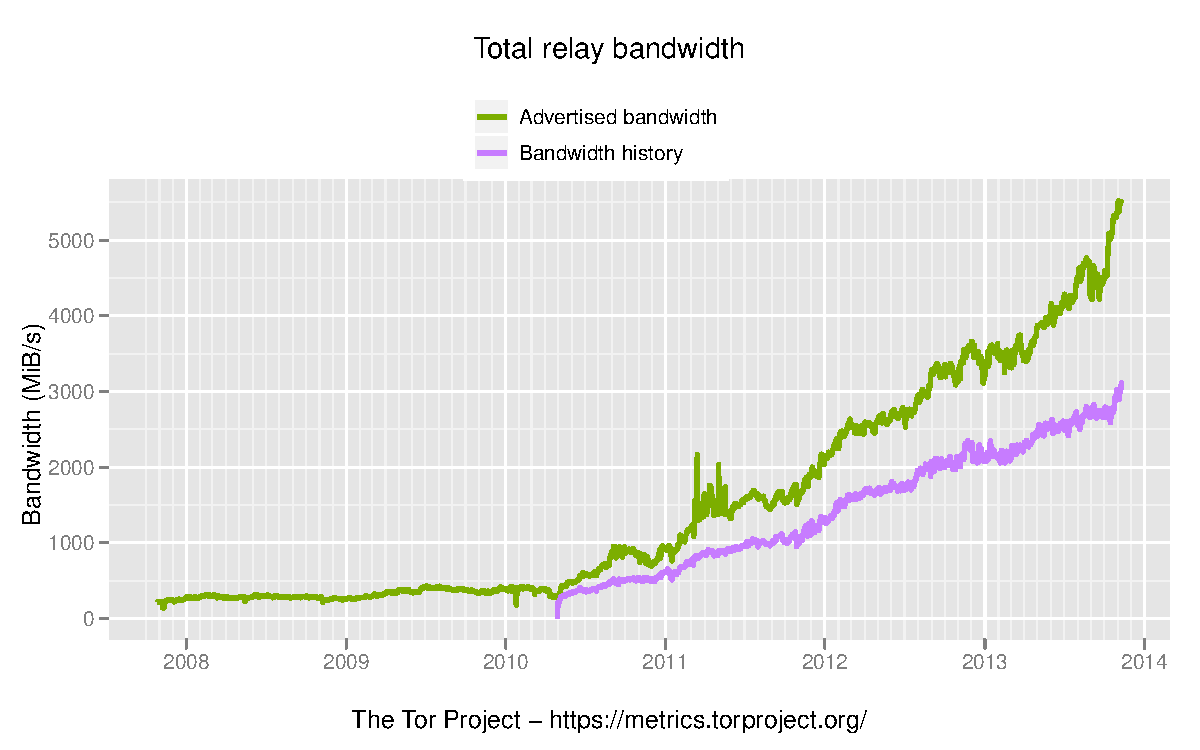
\includegraphics[width=0.7\textwidth]{bandwidth-2004-08-16-2013-11-14.pdf}
\caption{Tor Bandwidth Availability}
\label{fig:tor_bandwidth}
\end{figure}

However, Tor does have a robust design despite unstable relays.
Relays may be quite unstable and have short uptimes (in days).  The
Tor directory servers, in addition to listing the relays, also vote on
relay attributes and assign ``flags'' based on these attributes.  For
example, a router is listed as ``stable'' only if it meets a certain
Mean Time Between Failure (MTBF).  The impact of the stable flag is
that Tor clients are much more likely to choose stable relays.
Therefore the Quality of Experience (QoE) for the user should be
relatively consistent due to this incentive to choose stable relays.
Even as numerous volunteer relays enter and leave the
network, Tor provides an overall available service.

\subsection{Interoperability}

Tor provides a network service through an extenbility entry port: a
SOCKS proxy.  This entry point allows any application which conforms
to the SOCKS specification, access to the Tor network.  While Tor
itself runs as a daemon on the client machine, the proxy offers a
code-indepenent interface which has allowed various Tor projects to use
Tor services.

However, as Tor purpose is to provide IP anonymization, it is not
enough to simply use Tor as a SOCKS proxy.  For Tor to ``really
work,'' one has to ensure that DNS requests are not leaked in the clear
prior to using Tor.  As most applications were not built with privacy
in mind, Tor has forked Mozilla Firefox and distributes the fork as
the Tor Browser Bundle.  While Tor provides a clean interoperability
interface, to provide anonymity, there are significant challenges with
interoperability in existing software.

\subsection{Modifiability}

One of the fundamental architectural decisions of any network is
solving the discovery problem.  Tor relays are publically listed and
Tor directory services, while distributed, are the single point for
Tor relay discover.  This was successful at first, however, the
weakness in the client-server model had some challenges for Tor.
Specifically, it was trivial for Internet Service Provides to deny
access to Tor by blocking the IPs of all listed Tor relays.  This
effectivelly was a denial-of-service to Tor users.

Tor has some creative solutions around this problem.  It has since
introduced ``bridges'', basically private relays, as entry-points into
the Tor network.  Once one accesses a bridge, the user can use Tor
like normal.

While there is a tradeoff between client-server and peer-to-peer
discovery, in some sense the client server model makes Tor easier to
attack.  However, the adaptability of Tor's response to the attack
speaks well to it's modular architecture.

\subsection{Performance}

Tor was designed for low-latency application traffic like HTTP and
IRC.  However, even to the casual user, Tor is noticeably slower when
browsing the web.  Anonymity has a price and Tor traffic must make
three extra hops and contains three layers of encryption that must be
processed before reaching the destination.  Additionally, not all
relays provide the same level of QoS.

Therefore, Tor does not work well for high-bandwidth applications,
like BitTorrent.  Tor works reasonably well for media-lite web
traffic, but with increasing depth of content, the Tor network would
need more, faster relays to handle increased demand.

\subsection{Security}

Security is one of Tor's strongest points.  It has been design to be
resilient to attacks against anonymity.  Tor has several attributes of
good security engineering namely: Perfect Forward Security (PFS),
layered trust, and transparency.

Tor uses ephemeral key agreement algorithms in Transport Layer
Security (TLS) with routine key rotation.  Therefore, if a relay is
compromised and must turn over its keys, it will not compromise any
traffic that it has previously relayed.  Tor has a chain of trust
starting with the software.  The signed Tor software trusts a core set
of directory servers.  Those directory servers trust validated Tor
relays.  Therefore, Tor clients trust other Tor relays.  Lastly, Tor
is a free and open source project.  The security design, code, and
bugs are public and open for all to see.  This transparency encourages
independent reviews and trust in the project.



\subsection{Testability}

Testability is difficult metric for Tor.  As an anonymity network,
it is even difficult to collect usage data in a way that does not
compromise identities.  While individual software components have
tests, performing complicated test on the Tor network is discouraged.
Since individuals may be using Tor to protect their identity, a
researcher could unwillingly compromise their identity with a test.
Therefore, researchers are encouraged to construct isolated test
networks.

Since the core source is in C, Tor suffers from all of the normal
problems associated with cross platform support.  Furthermore, some
machines have specific cryptographic accelerators, further
complicating testing.  Tor produces release candidates and encourages
early adopters to run the software and then they watch the network
response.  Due to the unique anonymity requirements, testing appears
difficult for the Tor platform.

\subsection{Usabilility}

Security software is notoriously difficult to use.  However, Tor needs
volunteers to run relays and to a degree, the more diverse Tor is, the
better the anonymity.  Therefore Tor has spent significant effort
improving the usability.  Tor is one of the easiest security programs
to use.  One simply has to download the software and run it and the
Tor Browser Bundle will launch in a default configuration.  The
browser immediately directs to a webpage that informs the user if Tor
is working correctly.

Tor's commitment to usability is apparent in their decision to leave
Javascript enabled by default.  There are plenty of malicious
Javascript examples that could de-anonymize users or compromise their
security.  However, as most of the web uses Javascript, the Tor team
felt the adoptability would be low if Javascript was disabled.
Therefore it is on by default and users are made aware they can turn
it off if they desire.

\section{Conclusion}

Tor is a resilient and well architected platform.  Its strongest
qualities are security, modifiability, and usability.  For security
software, these are the three most critical attributes.  However, Tor's
architecture for scalability and performance provide some challenges.
As Tor continues to grow, it will be very interesting to see how Tor
adapts to accommodate additional users.  Overall, Tor is an excellent
example of a non-trivial, quality, architecture.

\section{References}

The following references were consulted in producing this architecture
summary:

\begin{itemize}
\item The Tor Protocol Specification:
  \url{https://gitweb.torproject.org/torspec.git?a=blob_plain;hb=HEAD;f=tor-spec.txt}
\item The Tor Directory Protocol, Version 3:
  \url{https://gitweb.torproject.org/torspec.git?a=blob_plain;hb=HEAD;f=dir-spec.txt}
\item The Tor FAQ: \url{https://www.torproject.org/docs/faq.html.en}
\item The Tor Source:
  \url{https://gitweb.torproject.org/tor.git/tree/refs/heads/master}
\item Tor mailing lists, where much of the development discussions are
  held: \url{https://lists.torproject.org/cgi-bin/mailman/listinfo}
\item Personal experience running a Tor relay.
\end{itemize}



\end{document}
% End of v2-acmlarge-sample.tex (March 2012) - Gerry Murray, ACM
